% ============================================================================
% Tests report: interpretation of the comparison (numbers from generado/comparacion/datos.tex).
% ============================================================================
\subsection{Lo observado}\label{sec:observado}

\paragraph{Los tres ensayos son reproducibles.} Con la misma cantidad de robots, la misma arena y el
mismo modo, las tres salidas dan estadísticas muy parecidas (\cref{tab:comparacion}): rapidez mediana
de \num{\Cmp{Vmed}{A}} a \SI{\Cmp{Vmed}{C}}{\milli\metre\per\second}, media de
\num{\Cmp{Vmean}{A}} a \SI{\Cmp{Vmean}{C}}{\milli\metre\per\second} y percentil 95 entre
\num{\Cmp{Vp95}{B}} y \SI{\Cmp{Vp95}{A}}{\milli\metre\per\second}; las distribuciones de rapidez y de
$\omega$ prácticamente se superponen (\cref{fig:cmp_hist}). La diferencia más grande entre ensayos no
está en cómo se mueven los robots cuando se mueven, sino en cuánto tiempo pasan atascados.

\paragraph{El movimiento es intermitente.} El percentil 95 de la rapidez es de cinco a seis veces la
mediana: la mayor parte del tiempo los robots apenas se desplazan (empujados por sus vecinos) y el
desplazamiento ocurre en episodios cortos de \num{3} a \SI{8}{\milli\metre\per\second}. A escalas de
1 a \SI{20}{\second}, el desplazamiento cuadrático medio crece como $\tau^{\alpha}$ con
$\alpha \approx \num{\Cmp{Alfa}{C}}$--$\num{\Cmp{Alfa}{A}}$, entre difusivo ($\alpha=1$) y balístico
($\alpha=2$): los robots mantienen la dirección durante algunos segundos. A tiempos largos el MSD se
satura (\cref{fig:cmp_giro}), porque el confinamiento limita el desplazamiento a la escala de la arena.

\paragraph{Sentido de giro y corrección del espejado.} Los videos están grabados espejados respecto del
eje vertical de la imagen, por lo que un giro horario real se ve antihorario. Todos los datos de este
informe están corregidos (opción \emph{Video espejado: horizontal} de VidFetch): ángulos y posiciones
corresponden a la arena vista desde arriba, con giros positivos en sentido antihorario.

\paragraph{La rotación propia domina.} Todos los robots giran sobre sí mismos de forma persistente:
la $|\omega|$ mediana es de \num{\Cmp{Wmed}{A}} a \SI{\Cmp{Wmed}{B}}{\degree\per\second} y el robot
más rápido acumula \num{\Cmp{Vmax}{C}} vueltas en \SI{\Cmp{Dur}{C}}{\minute} (una $|\overline{\omega}|$
de \SI{\Cmp{Spin}{C}}{\degree\per\second}). En el modo \texttt{QR} todos los robots están programados
para girar a la derecha (sentido horario), y eso es lo que hace la mayoría: en los tres ensayos,
\Cmp{Ncw}{A} robots giraron en neto en sentido horario y el giro medio con signo es negativo, de
\num{\Cmp{Wmean}{B}} a \SI{\Cmp{Wmean}{C}}{\degree\per\second}.

\paragraph{Contrarrotación de los robots de la pared.} Los otros \Cmp{Nccw}{A} robots terminan con un
giro neto antihorario, contrario al programado (\cref{fig:cmp_giro}, izquierda). No son simplemente
robots que fallan: giran despacio ($|\overline{\omega}| \approx \SI{2}{\degree\per\second}$, contra
\num{5}--\SI{6}{\degree\per\second} de los que giran a la derecha), alternan ambos sentidos (giran a la
derecha el \num{40}--\SI{47}{\percent} del tiempo) y pasan más tiempo contra la pared
(\num{58}--\SI{68}{\percent} del tiempo con $r/R_{\mathrm{c}} > 0{,}85$, contra \num{47}--\SI{52}{\percent}).
Esto es lo que se espera de un disco que rueda por el interior de la pared: si avanza en sentido
horario alrededor del centro de la arena apoyado en ella, el rozamiento en el punto de contacto lo hace
girar en sentido antihorario sobre sí mismo, y ese arrastre puede superar al giro propio del motor.
La coincidencia 14/8 en los tres ensayos sugiere además que la tendencia depende de cada robot (por
ejemplo, de la fuerza de su motor); para confirmarlo haría falta identificar a cada robot entre videos,
cosa que el seguimiento no hace.

\paragraph{Hay una circulación colectiva débil.} El parámetro
$\Phi = \langle \hat r_i \times \hat v_i \rangle$ (seno del ángulo entre la posición respecto del
centro de la arena y la velocidad, promediado sobre los robots que se mueven a más de
\SI{1}{\milli\metre\per\second}) vale \num{\Cmp{Prot}{A}}, \num{\Cmp{Prot}{B}} y \num{\Cmp{Prot}{C}}:
valdría $-1$ si todos circularan en sentido horario alrededor del centro, $+1$ en sentido antihorario
y 0 si no hubiera sentido preferido. El grupo circula lentamente en sentido horario, el mismo sentido
del giro programado, con una velocidad angular colectiva de unos \SI{0.2}{\degree\per\second} (una
vuelta cada \SI{30}{\minute}).

\paragraph{Los robots se ordenan en capas.} Los mapas de ocupación (\cref{fig:cmp_ocupacion}) y la
densidad radial (\cref{fig:cmp_radial}) muestran tres anillos concéntricos en $r/R_{\mathrm{c}} \approx
0{,}14$, $0{,}55$ y $0{,}95$, separados por aproximadamente un diámetro de robot. La capa exterior,
apoyada en la pared, es la más poblada; entre la capa media y la exterior la densidad cae a
\num{0.15}--\num{0.4} veces el valor uniforme. Es el ordenamiento esperado de discos densos en un recinto circular ($\phi \approx 0{,}58$):
los robots se reacomodan dentro de cada capa y pasan poco tiempo entre capas.

\paragraph{Atascos.} Los tres ensayos tienen intervalos en los que todo el grupo se detiene
(\cref{fig:cmp_serie,fig:atascos}): la rapidez de casi todos los robots cae al nivel del ruido de posición
(mediana $\approx\SI{0.2}{\milli\metre\per\second}$) y la rotación propia también se frena, de
$|\omega| \approx \SI{4}{\degree\per\second}$ a menos de \SI{1.5}{\degree\per\second}. No es una pausa de los
robots: siguen encendidos (los LEDs se ven en el video) y el movimiento se reanuda solo. \Cmp{Lab}{A} es
el ensayo más afectado: \Cmp{NAt}{A} atascos que suman \SI{\Cmp{TAt}{A}}{\minute}
(\SI{\Cmp{PAt}{A}}{\percent} del ensayo), uno de \SI{\Cmp{AtMax}{A}}{\second} entre los minutos 45 y 51,
y otro que dura desde el minuto 62 hasta el final. \Cmp{Lab}{B} tuvo un único atasco de
\SI{\Cmp{AtMax}{B}}{\second} y \Cmp{Lab}{C}, \Cmp{NAt}{C} cortos (\SI{\Cmp{TAt}{C}}{\minute} en total).
Fuera de los atascos, la rapidez mediana de los tres ensayos es casi igual
(\num{\Cmp{VmedAct}{B}}--\SI{\Cmp{VmedAct}{C}}{\milli\metre\per\second}).

\begin{figure}[H]
  \centering
  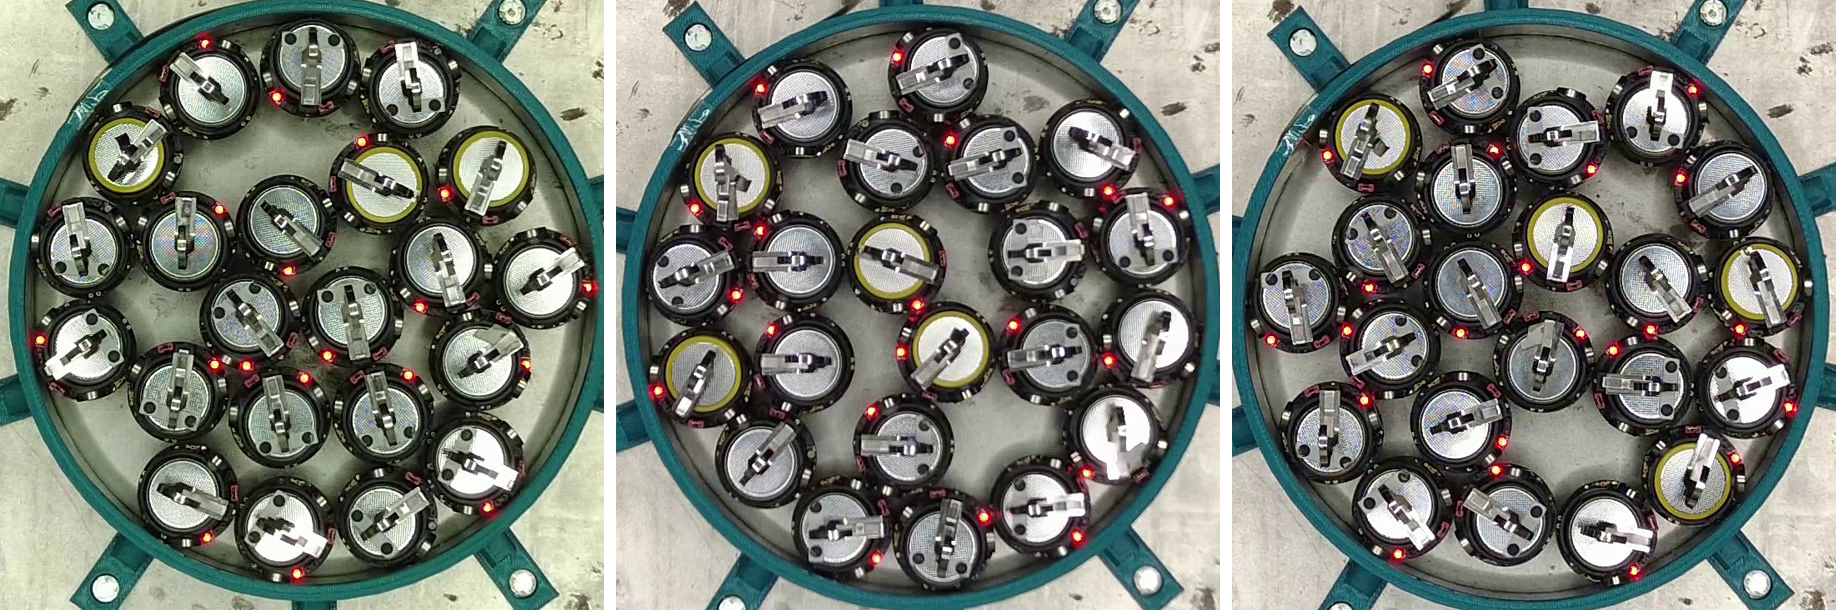
\includegraphics[width=\linewidth]{figuras/atascos.png}
  \caption{Un cuadro durante el atasco principal de cada ensayo (de izquierda a derecha: \Cmp{Lab}{A},
    minuto 47,8; \Cmp{Lab}{B}, minuto 50,6; \Cmp{Lab}{C}, minuto 19,7). Imágenes tal como las graba la cámara (espejadas). Los robots siguen
    encendidos (LEDs rojos), pero durante el atasco prácticamente no se desplazan ni giran.}
  \label{fig:atascos}
\end{figure}
